\section{Experiments}

\begin{table}[!tb]
  \centering
  \begin{tabular}{|c|c|c|}
    \hline
      & \textbf{1-Hot Labels} & \textbf{Word2Vec Labels} \\
    \hline
      \textbf{VGG-16} & 0.2167 & 0.2091 \\
    \hline
      \textbf{4-layer CNN} & 0.1091 & 0.1864 \\
    \hline
  \end{tabular}
  \caption{
    The training results after 50 epochs of using 1-hot labels vs. using soft
    labels from Word2Vec.
  }
  \label{tbl:results}
\end{table}



We will evaluate and compare the performance of deep convolutional neural
networks trained on ImageNet with soft labels and 1-hot labels.
We will train the VGG-16 model \cite{simonyan2014very} from scratch, and see
how well it learns using the different labeling schemas. Our goal is to try to
find the optimal hyperparameters for which soft label training will outperform
1-hot labels.
We will also analyze the errors made by both models to see how semantically
relevant the models are.
We plan to use the evaluation method introduced in \cite{zhao2011large} for
testing semantically relevant errors.

We will also experiment with pretrained networks and different architectures to
see how effectively they can learn with soft labels compared to 1-hot labels.
In \cite{hinton2015distilling} the authors showed that they can use soft labels
to train simpler models quickly that perform nearly as well as the advanced
models with many more parameters. We hope to mirror these results, but using
semantic weights for the learning targets.
Finally, we plan to experiment with training on fewer examples to see if our
approach can help in cases where labeled data is limited.

Throughout all of our experiments, we will compare different schemes for
obtaining the soft labels. We will use Word2Vec, WordNet, and possibly visual
similarity, and discover optimal distributions for these weights.
We hope to look at different linguistic semantic similarity measures and
compare them with visual similarity measures, and analyze which object
categories relate well in both the visual and semantic domain.



\begin{figure}[!tb]
%\begin{figure}[t]
  \centering
  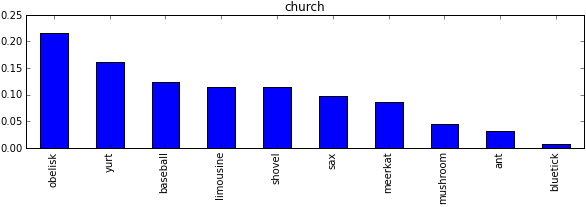
\includegraphics[width=0.5\textwidth]{figs/word2vec_church.png}
  \caption{
    The Word2Vec similarity scores for \emph{church}. Other structures, such as
    \emph{obelisk} and \emph{yurt} (a type of tent) were the closest in
    similarity. \emph{Bluetick} (a type of dog) was the most distant.
  }
  \label{fig:word2vec_similarities}
\end{figure}

As a proof of concept, we trained two models on a small amount of data from
ImageNet. We used 11 ImageNet classes -
\emph{
  saxophone,
  limousine,
  shovel,
  baseball,
  meerkat,
  church,
  yurt,
  obelisk,
  bluetick,
  mushroom,
  ant
} -
each with 100 training examples and 20 test examples.
Using Word2Vec trained on articles from Google News, we extracted similarity
scores between these categories. The similarity scores for \emph{church} are
shown in Figure \ref{fig:word2vec_similarities}.

We trained the VGG-16 model as well as a simpler four-layer CNN on this data
set. Our average results over three experimental trials can be seen in Table
\ref{tbl:results}.
While the results for the VGG-16 model are similar in both cases, there is a
clear boost in performance on the simpler model. Our naivly-selected soft
labels perform almost as well as VGG-16 despite being a significantly inferior
architecture.
The overall poor performance can be attributed to the tiny training data set.

Naturally, we will run experiments with much larger training sets and we will
search for the best hyperparameters.
We will also work on improving the design of the soft labels, which were not
adjusted at all for this experiment - we just took the cosine similarity
between the raw Word2Vec features.



%\subsection{CNN Architecture}
%
%TODO.
